\section{HTML5}

Für die Implementierung der Browseranwendung wird auf den aktuellen Entwurf des  zukünfitgen HTML5
Standards zurückgegriffen. \cite{html5}

\acr{html} ist eine Sprache die der strukturierten  Beschreibung von Webseiten dient. Die Sprache
wurde in ihrer ursprünglichen Form  von 1989-1992, lange vor dem sogenannten Web 2.0, von
Wissenschaftlern des  Europäischen Kernforschungsinstitut CERN entwickelt. Sie war der erste nicht
proprietäre globale Standard zur digitalen übertragung von Strukturierten  Dokumenten. Die Sprache
\acr{html} allein ist nicht geeignet um dynamische Inhaltem  wie sie heute praktisch auf allen
modernen Webseiten vorkommen, zu beschreiben.

Der heutige HTML5-Standard geht weit über die Sprache \acr{html} selbst hinaus und  umfasst vor
allem auch die Scriptsprache \acr{js} und die darin verfügbaren  Bibliotheken, sowie das
sogenannte \acr{dom}, auf welches in  Scripten zugegriffen werden kann um den angezeigten Inhalt
dynamisch zu  verändern.

\subsection{Dokumenobjektmodell}

Das \acr{dom} ist eine Schnittstelle, die es Erlaubt \acr{html}- bzw. \acr{xml}-Dokumente zu
modifizieren und bildet damit die Grundlage für die Realisierung dynamischer Webseiten.

Der Einstiegstpunkt in das \acr{dom} ist der \texttt{document} Knoten, welcher von in \acr{js}
global verfügbar ist und von welchem aus die gesamte Baumstruktur erreichbar ist. Jeder
\acr{html}-Tag, jedes Attribut und jeder Text wird als ein Objekt, bzw. ein Knoten im Baum
repräsentiert. Über verschiedene Methoden ist es möglich die Kinder-, Geschwister- und Elternknoten
zu erhalten. Durch funktionen wie z.B. \texttt{appendChild} ist es schließlich möglich neue Elemente
in das \acr{dom} zu integrieren bzw. bestehende zu modifizieren. \cite{dom}

\subsection{Cascading Styles Sheets}

\acr{css} ist eine Sprache die der Definition von  Stilen bzw. Stilvorlagen für die Anzeige von
Webinhalten dient.

Durch die Trennung von \acr{html} und \acr{css} wird erreicht, dass \acr{html}-Dokumente sich auf
den Inhalt einer Seite beschränken, während alle die grafische Anzeige  belangenden Aspekte in die
sogenannten Stylesheets in \acr{css} Dateien ausgelagert  werden.

\subsubsection{CSS3}

In der kommenden \acr{css} Version 3.0, welche bereits zu großen Teilen von den meisten aktuellen
Browsern unterstützt wird kommen einige interesante Neuerungen hinzu welche es vor allem
Ermöglichen, Anwendungen welche man Bisher in Frameworks wie Flash oder Silverlight implementiert
hat nun in reinem \acr{html}+\acr{css} zu verwirklichen. Die für die Realisierung der
brwoserbasierten Entwicklungsumgebung relevanten Neuerungen umfassen im speziellen

\begin{itemize}
  \item Einbetten von Schriftarten,
  \item Animationen und Übergänge,
  \item Verhindern von Textmarkierungen und
  \item Festlegen der Sichtbarkeit von Elementen für den Mauszeiger.
\end{itemize}

\subsubsection{LESS}

\label{sec:less}

Auch \acr{css}3 hat immernoch einige konzeptionell Einschränkungen welche die Arbeit damit stark
erschweren:

\begin{itemize} 
  \item Es ist nicht möglich Variablen zu definieren um Eigenschaften, welche an
vielen Stellen vorkommen nur einmal zu definieren. 
  \item Es fehlen Funktionsdefinitonen um ähnliche
oder abhängige Definitionen  zusammenzufassen und zu parametrisieren. 
  \item Die Hierarchie einer
\acr{css}-Datei ist flach obwohl die Definitionen geschachtelt sind. Das reduziert die lesbarkeit
der Dateien. 
  \item Wenn aus Gründen der Übersichtlichkeit \acr{css} in mehrere Dateien aufgeteilt
werden, müssen alle Dateien einzeln geladen werden, was zu längeren Ladezeiten führt. \end{itemize}

\textit{LESS} ist eine Erweiterung von \acr{css} welche unter anderem  Variablen- und
Funktionsdefinitionen, verschachtelte Definitionen sowie  Dateiimports erlaubt. Damit werden die
oben genannten Einschränkungen von \acr{css} aufgehoben.

Das Play Framework (Siehe Abschnitt \ref{sec:play}) ermöglicht es die Stylesheet-Sprache
\textit{LESS} zu verwenden ohne,  dass diese auf Browserseite unterstützt werden muss. Hierfür
werden die in  \textit{LESS} definierten Stylesheet auf Serverseite in \textit{CSS} übersetzt  und
dem Browser zur Verfügung gestellt. Dafür müssen die Dateien an einem vorher konfigurierten Ort
liegen. Nach dem  übersetzen werden sie an der selben Stelle zur Verfügung gestellt wie normale
\textit{CSS} Dateien.

\subsection{JavaScript}

\acr{js} ist eine dynamisch typisierte, klassenlose objektorientierte Scriptsprache welche aktuell
der Standard in der Entwicklung von clientseitigem Code für dynamische Webinhalte ist. Der Kern von
\acr{js} wurde von der Ecma International als ECMAScript normiert. Durch \acr{js} ist es
möglich Webseiten dynamisch zu verändern. Siehe auch \cite{js}.

\subsubsection{CoffeeScript}
\label{sec:coffeescript}

\acr{js} wurde in Eile entwickelt und normiert, da zur Zeit der Entstehung ein schneller Bedarf an
einer normierten Sprache für das Web bestand. Dadurch sind jedoch auch einige Unschönheiten in den
Sprachkern gedrungen. So ist beispielsweise die C-artige Syntax für eine eher funktional angehauchte
Sprache wie \acr{js} ungeeignet, da Funktionsdefinitonen durch geschweifte Klammern, das
Schlüsselwort \texttt{function} und ein \texttt{return} Statement unnötig aufgeblasen werden und
damit unleserlicheren Code erzeugen. Darüber hinaus fehlt in \acr{js} jede Möglichkeit der
Modularisierung. Da noch nicht einmal Klassen existieren, führt das bei reinem JavaScript schnell zu
unwartbarem Code. Ein weiterer Stolperstein ist das Schlüsselwort \texttt{this} welches nicht immer
klar zu verstehen ist, da es in Funktionsaufrufen seine bedeutung wechseln kann.

textit{CoffeeScript}\footnote{http://www.coffeescript.org} ist eine neue Scriptsprache mit dem Ziel
die Unschönheiten von \acr{js} auszumärzen. CoffeeScript hat eine eher an funktionale Sprachen wie
Haskell erinnernde Syntax mit Verschachtelungen über Whitespace und einem \texttt{->} Operator zur
Funktionsdefinition. Darüber hinaus bietet CoffeScript die Möglichkeit Klassen zu definieren und
führt das Konzept der Vererbung ein. Das \texttt{this}-Schlüsselwort kann an Instanzen von Klassen
gebunden werden. CoffeeScript Dateien werden zu optimiertem \acr{js} Code kompiliert, welcher den
Vorgaben des \textit{\acr{js} Linter}\footnote{http://www.javascriptlint.com/} entspricht. Im
einzelnen sind die Verbesserungen gegenüber \acr{js}:

\begin{itemize}
  \item Vereinfachte Syntax für Funktionsdefinitionen, Arrays, Blöcke,
  \item automatisches initialisieren von Variablen (\textit{lexical scoping}),
  \item \textit{Splats} (Variable Parameterlisten),
  \item universellere Iterationsschleifen (\texttt{for}),
  \item vereinfachtes \textit{slicing} und \textit{splicing} (Arrayoperationen),
  \item Ausdrucksorientiertheit,
  \item Klassen und Vererbung,
  \item ein Existenzoperator,
  \item destrukurierende Zuweisungen (z.B. \texttt{[a,b] = [c,d]}),
  \item Bindung von \texttt{this} an Klasseninstanzen sowie
  \item mehrzeilige Strings und reguläre Ausdrücke mit Kommentaren
\end{itemize}

Genauso wie für \textit{LESS} existiert im Play Framework (Siehe Abschnitt \ref{sec:play}) die
Serverseitige Unterstützung  für \textit{CoffeeScript}. Die in CoffeeScript geschriebenen
Dateien  werden ebenfalls an gleicher Stelle wie normale \acr{js}-Dateien dem  Browser
als \acr{js} zur Verfügung gestellt.


\subsection{HTTP}

\acr{http} \TODO{HTTP}

\subsubsection{AJAX}

\acr{ajax} ist keine Bibliothek und auch kein  Standard sondern ein sehr
weit verbreitetes Konzept zur Übertragung von Daten  zwischen Browser und Webserver. Hierbei wird
das \acr{js}-Objekt \texttt{XMLHttpRequest} verwendet um während der Anzeige einer Webseite

\begin{figure}[ht]
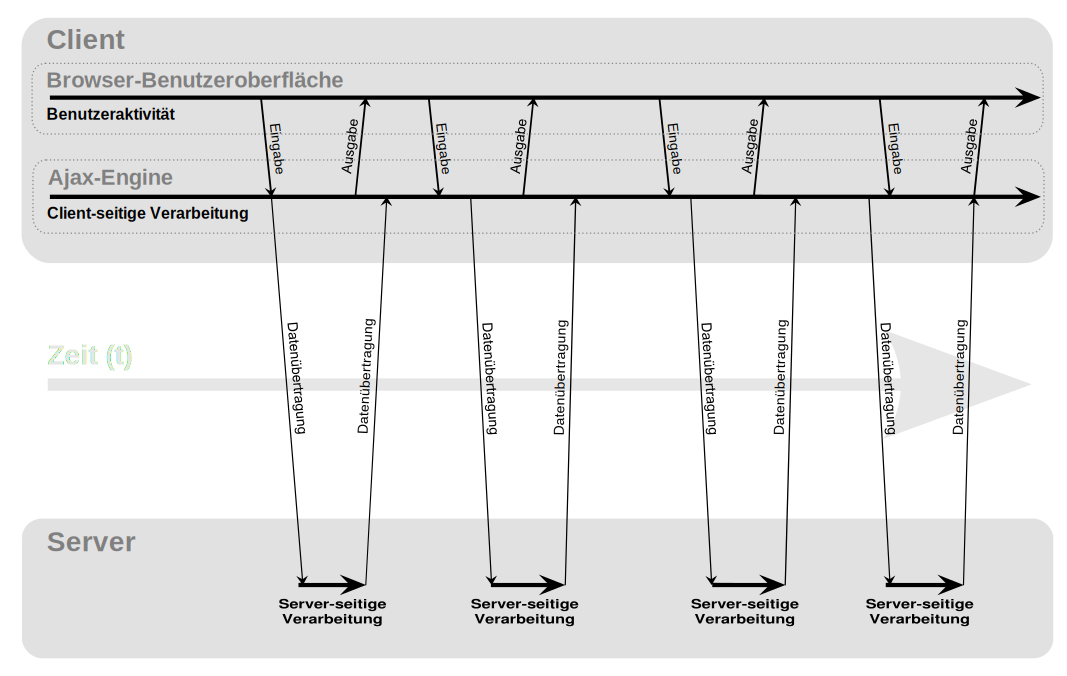
\includegraphics[width=\linewidth]{images/diagram-ajax}
  \caption{Ajax Modell einer Web-Anwendung (asynchrone Datenübertragung)}
  \captionsetup{font={footnotesize,bf,it}}
  \caption*{Quelle: Wikipedia}
  \label{fig:diagram-ajax}
\end{figure}

\TODO{AJAX}

\subsubsection{WebSockets}

Websockets sind ein in HTML5 neu eingeführter Standard zur bidirektionalen  Kommunikation zwischen
Browser und einem Webserver. Hierbei wird anders als bei  AJAX eine direkte TCP-Verbindung
hergestellt. Diese Verbindung kann sowohl von  Browser- als auch von Serverseite aus gleich
verwendet werden. Das macht es  unnötig, wie bei AJAX wiederholte Anfragen oder Anfragen ohne
Zeitbegrenzung zu  stellen um Informationen vom Server zu erhalten wenn diese Verfügbar werden. Ein
weiterer Vorteil gegenüber HTTP-Anfragen ist, dass durch die direkte permanente Verbindung kein
Nachrichtenkopf mehr nötig ist. Das macht es deutlich  effizienter viele kleine Nachrichten zu
versenden. \TODO{WebSockets}

\subsection{JavaScript-Bibliotheken}

Über den HTML5 Standard hinaus werden für die strukturierung der Anwendung einige
\acr{js}-Bibliotheken verwendet, welche im folgenden kurz erläutert werden.

\subsubsection{jQuery}

Die Bibliothek \textit{jQuery} ist ein defacto Standard in der Webentwicklung.  In erster Linie
erleichtert es den Zugriff auf das \textit{DOM}. \TODO{jQuery}

\subsubsection{Backbone und Underscore}

\textit{Backbone} ist eine Bibliothek, die der Strukturierung von acr{js} Anwendungen dient und baut
auf der 

\subsubsection{RequireJS}
\label{sec:requirejs}

Da JavaScript von Haus aus keine Möglichkeit der Modularisierung bietet, komplexe Anwendungen
jedoch ohne Modularisierung kaum wartbar bleiben, haben sich unterschiedliche Lösungsansätze für
dieses Problem entwickelt. Einer der  umfassendsten ist die Bibliothek \textit{RequireJS}.

Mit der Funktion \texttt{define} können Module in Form von Funktionsdefinitionen  definiert werden.
Alle lokalen Variablen in dem Modul sind anders als bei  normalen Scripten außerhalb nicht mehr
sichtbar, da sie innerhalb einer  Funktion definiert wurden. Das Funktionsergebnis ist das was nach
außen Sichtbar  ist. Das kann ein beliebiges Objekt (also auch eine Funktion) sein.

Die so definierten Module können Abhängigkeiten untereinander spezifizieren  indem der
\texttt{define}-Funktion eine Liste von Modulen übergeben wird, die  das aktuelle Modul benötigt.
Die \textit{RequireJS}-Bibliothek sorgt dann dafür,  dass diese Module geladen wurden bevor das
aktuelle Modul ausgeführt wird.

RequireJS bietet die Möglichkeit den  \acr{js}-Code für den Produktiveinsatz zu optimieren. Dafür
gibt es  das sogenannte \textit{r.js}-Script welches unter andem alle Abhängigkeiten in eine Datei
zusammenfasst und den Code durch das Entfernen von Whitespaces und Kommentaren  sowie dem Umbenennen
von Variablennamen verkürzt. Zur Entwicklungszeit ist dieser nicht mehr lesbare Code nicht
erwünscht. Deswegen bietet das Play Framework (Siehe Abschnitt \ref{sec:play}) eine integrierte
Version von RequireJS, welche automatisch den lesbaren Code zur Entwicklungszeit  bereitstellt, im
Produktiveisatz jedoch den optimierten.
